\documentclass[a4paper,10pt]{article}
\usepackage[utf8]{inputenc}
\usepackage{amsfonts,amssymb}
\usepackage{color}
\usepackage[table]{xcolor}
\usepackage{tikz}
\usepackage{pgfplots}
\usepgfplotslibrary{fillbetween}
\usetikzlibrary{positioning,fadings,arrows,babel}
\usetikzlibrary{tikzmark,decorations.pathreplacing}
\pgfplotsset{width=10cm,compat=1.9}
\usepgfplotslibrary{fillbetween}

\begin{document}

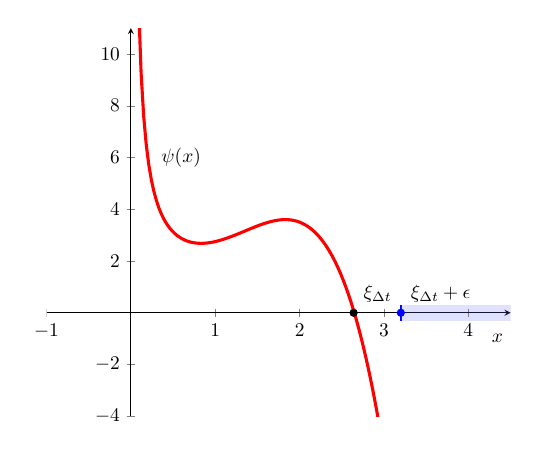
\begin{tikzpicture}[scale=0.7]
\begin{axis}[
	    axis lines = center,
	    ymin=-4, ymax=11,
	    xmin=-1, xmax=4.5,
	]
	\addplot [
	    domain=0:3, 
	    samples=100, 
	    color=red,
	    ultra thick
	]
	{1+(1/x)-((x^4)/2)+((5*x^3)/4)};
	\draw[blue, very thick] (axis cs:3.2,-0.3) -- (axis cs:3.2,0.3);
	\fill[color = blue!60, opacity=0.2] (axis cs:3.2,-0.3) rectangle (axis cs:4.5,0.3);
	\node[label={45:{$\xi_{\Delta t}$}},circle,fill,inner sep=1.5pt] at (axis cs:2.64,0) {};
	\node[blue,label={45:{$\xi_{\Delta t}+\epsilon$}},circle,fill,inner sep=1.5pt] at (axis cs:3.2,0) {};
	\node[label={265:{$x$}}] at (axis cs:4.5,-0.3) {};
	\node[label={0:{$\psi(x)$}}] at (axis cs:0.2,6) {};
	\end{axis}
	\end{tikzpicture}

\end{document}